%**************************************************************************************
\section{Phenomenology and Modeling of Bottom Reflood}\label{sec:reflood_phenomenology}
%**************************************************************************************

% Opening Paragraph, the reflood phase 
\emph{Reflood} phase is the last phase of the $4$ canonical phases in the mitigation of \gls[hyper=false]{lbloca} in a \gls[hyper=false]{pwr}; the other $3$ preceding phases are \emph{blowdown} phase, \emph{refill} phase, and \emph{bypass} phase (see \cite{Hewitt2000} for an introduction on the transient).
It refers to the phase of the transient at which emergency coolant water flows slowly upward through the reactor core quenching the fuel elements along the way. 
The phase occurs after a successful injection of the water through the downcomer and lower plenum of the \gls[hyper=false]{rpv} (i.e., the refill phase).

% Reflooding
\emph{Quenching} (or \emph{rewetting}) refers to the phenomenon in which a contact between the liquid phase of the coolant and the hot surface of the fuel elements.
Prior to the quenching, the excessively high surface temperature prevents a stable contact between the liquid phase and the surface, degrading the \gls[hyper=false]{ht} between the two.
The maximum temperature for which the liquid might make a stable contact with the surface is referred to as the \emph{quenching} temperature.
In consequence, although the bulk of the flow through the core is liquid, the inability for the liquid to make contact with the surface keeps the surface temperature at a very high level \cite{Hewitt2000,Zeng2010}.

In \gls[hyper=false]{bwr} type reactors, reflood might also occurs by spraying the core from the top resulting in the \emph{top reflood};
while in both \gls[hyper=false]{bwr} and \gls[hyper=false]{pwr} type reactors, injection of water downward through the downcomer and upward through the core is termed \emph{bottom reflood}.
There are different physical processes associated with the two, such as the fact that in the top reflood there is steam flow from the bottom of the channel pushing back the liquid injection.
This thesis only concern with the bottom reflood. 
As the process set a limiting ability for the emergency coolant to bring about efficient cooling to the fuel elements in the \gls[hyper=false]{lbloca} transient, a proper modeling of the physical processes associated with the reflood phase is an important for the safety analysis of \glspl[hyper=false]{lwr}.

% Reflood curve
A typical mid-height cladding temperature evolution in a channel undergoing a bottom reflood (so-called \emph{reflood curve}) can be seen in Fig.~\ref{fig:ch2_reflood_curve_qois} under a constant coolant injection rate and a constant power boundary condition.
At the start of the transient (cladding temperature at $T_\text{init.}$) the channel is consists purely of steam flow.
Keeping the power constant increases the cladding temperature up until a mixture of steam and liquid (droplets) arrives at the location, improve the \gls[hyper=false]{ht} mechanism, and turn the temperature around from the maximum ($T_\text{max.}$).
As the channel keeps undergoing reflood from the bottom, more droplets are available at the location to keep decreasing the cladding temperature.
Finally, when the temperature of the cladding reaches the quenching temperature ($T_\text{quench}$), quenching occurs and stable contact between liquid and the cladding can be established.
From that point onward, the cladding temperature is in equilibrium with the liquid at saturation.
\begin{figure}[bth]
    \centering
    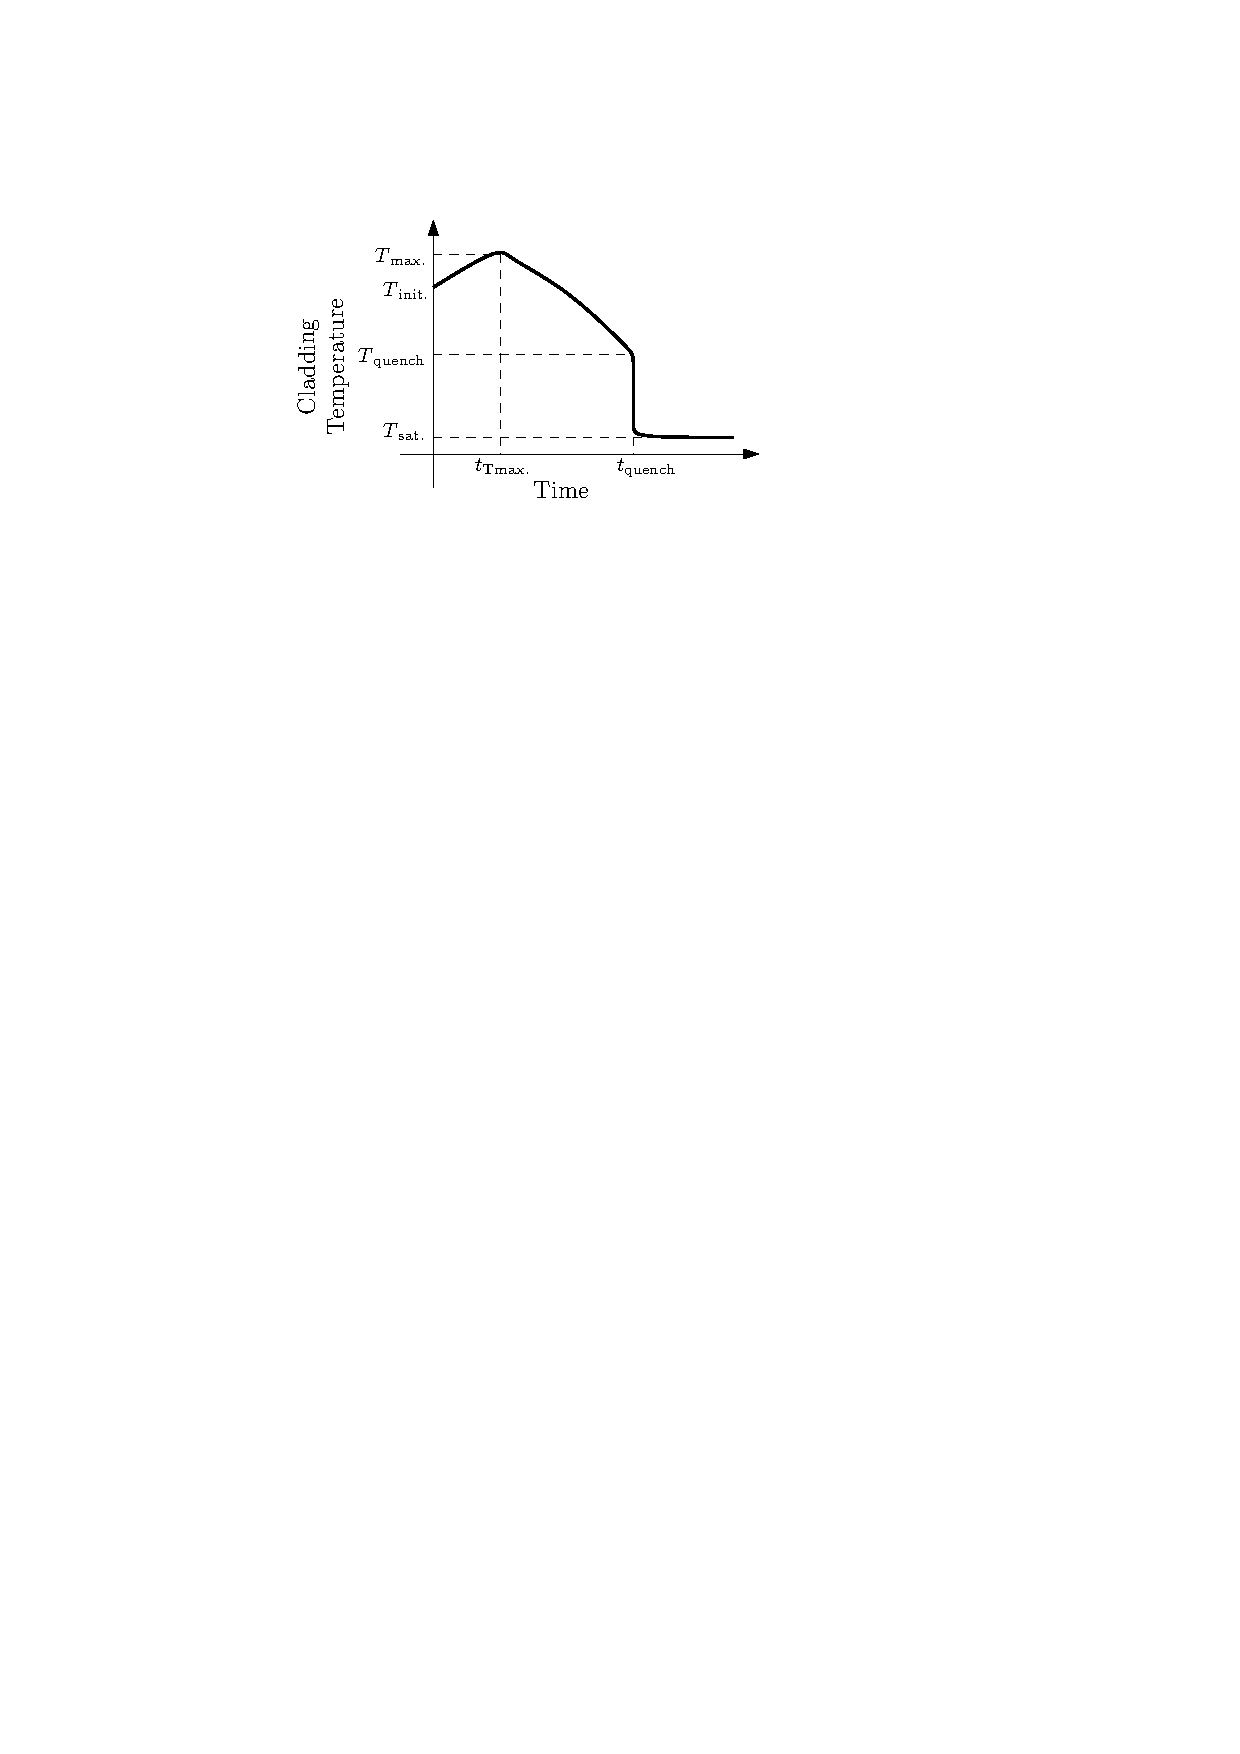
\includegraphics[width=1.0\textwidth]{../figures/chapter2/figures/refloodCurveQoIs}
    \caption[A typical cladding temperature evolution during constant flooding rate reflooding at mid-height assembly.]{A typical cladding temperature evolution during constant flooding rate reflooding at mid-height assembly (adapted from \cite{Zeng2010}). The labels on the both axes are typical \glspl[hyper=false]{qoi} of reflood transient, where the abbreviations $max.$, $init.$, and $sat.$ refer to the \emph{maximum}, \emph{initial}, and \emph{saturation}, respectively.}
    \label{fig:ch2_reflood_curve_qois}
\end{figure}

% The Modeling of The Phenomenology
Phenomenological view of the process, as adopted by \gls[hyper=false]{trace} code, is shown in Fig.~\ref{fig:ch2_reflood_phenomenology} along with the corresponding part in the reflood curve Fig.~\ref{fig:ch2_reflood_curve}.
The post-\gls[hyper=false]{chf} flow regimes (regimes $(2)$--$(5)$ in the figure) are in between two pre-\gls[hyper=false]{chf} regimes and pure steam convection.
\normdoublefigure[pos=h,
                  mainlabel={fig:ch2_reflood_phenomenology},
                  maincaption={Phenomenology of flow during reflood according to \gls[hyper=false]{trace} code and the corresponding .},
				mainshortcaption={Phenomenology of flow during reflood according to \gls[hyper=false]{trace} code.},
                  leftopt={width=0.45\textwidth},
                  leftlabel={fig:ch2_reflood_curve_phenomenology},
                  leftcaption={post-\gls[hyper=false]{chf} flow regimes $(2)$--$(5)$},
                  %leftshortcaption={},%
                  rightopt={width=0.5\textwidth},
                  rightlabel={fig:ch2_post_chf_regime},
                  rightcaption={Reflood curve}]
{../figures/chapter2/figures/postCHFRegime}
{../figures/chapter2/figures/refloodCurvePhenomenology}
